\documentclass[12pt,a4paper]{article}
\usepackage[utf8]{inputenc}
\usepackage[T1]{fontenc}
\usepackage{amsmath}
\usepackage{amsfonts}
\usepackage{amssymb}
\usepackage{graphicx}
\usepackage{hyperref}
\usepackage{xcolor}
\usepackage{tikz}
\usepackage{pgfplots}

\title{Probability Distributions}
\author{Rayan El Idrissi}
\date{\today}

\begin{document}

\maketitle
\tableofcontents
\newpage

\section{Historical Development}
\subsection{1713: Binomial distribution}
Jacob Bernoulli's "Ars Conjectandi," published posthumously in 1713, introduced the binomial distribution and contained the first version of the law of large numbers.

\subsection{1837: Poisson distribution}
Siméon Denis Poisson developed what is now known as the Poisson distribution in his work "Recherches sur la probabilité des jugements en matière criminelle et en matière civile."

\subsection{1925: Statistical distributions theory}
Ronald Fisher made significant contributions to modern statistical theory, including maximum likelihood estimation and the development of exact sampling distributions.

\section{Discrete Probability Distributions}
\subsection{Bernoulli Distribution}
The Bernoulli distribution models an experiment with exactly two possible outcomes, "success" (probability $p$) and "failure" (probability $1-p$). The probability mass function (PMF) is:

\begin{align}
P(X = x) = \begin{cases}
p, & \text{if } x = 1 \\
1-p, & \text{if } x = 0
\end{cases}
\end{align}

Expected value: $E[X] = p$\\
Variance: $\text{Var}(X) = p(1-p)$

\subsection{Binomial Distribution}
The binomial distribution models the number of successes in $n$ independent Bernoulli trials, each with probability $p$ of success:

\begin{align}
P(X = k) = \binom{n}{k} p^k (1-p)^{n-k}, \quad k = 0, 1, 2, \ldots, n
\end{align}

Expected value: $E[X] = np$\\
Variance: $\text{Var}(X) = np(1-p)$

\subsection{Poisson Distribution}
The Poisson distribution models the number of events occurring in a fixed interval of time or space, when these events occur with a known constant mean rate and independently of each other:

\begin{align}
P(X = k) = \frac{\lambda^k e^{-\lambda}}{k!}, \quad k = 0, 1, 2, \ldots
\end{align}

Expected value: $E[X] = \lambda$\\
Variance: $\text{Var}(X) = \lambda$

\subsection{Geometric Distribution}
The geometric distribution models the number of trials needed to get the first success in repeated independent Bernoulli trials:

\begin{align}
P(X = k) = (1-p)^{k-1} p, \quad k = 1, 2, 3, \ldots
\end{align}

Expected value: $E[X] = \frac{1}{p}$\\
Variance: $\text{Var}(X) = \frac{1-p}{p^2}$

\begin{figure}[h]
\centering
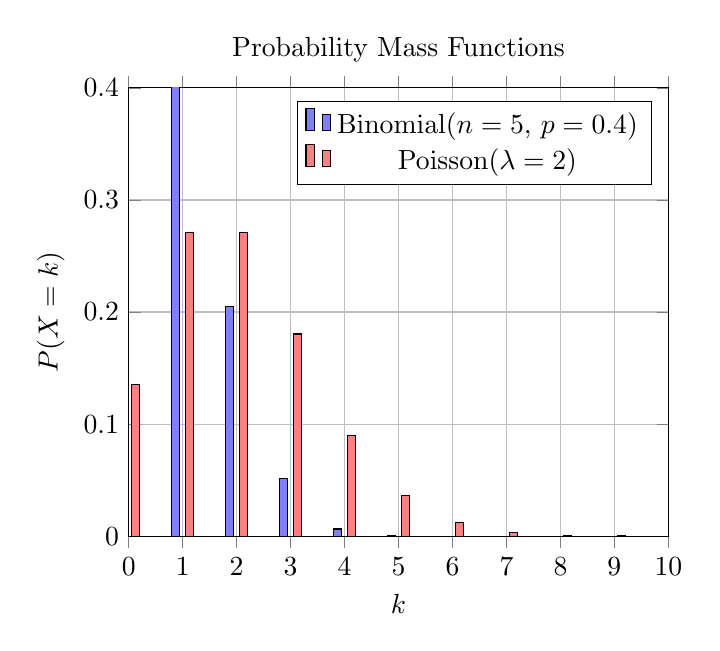
\begin{tikzpicture}
\begin{axis}[
    xlabel={$k$},
    ylabel={$P(X=k)$},
    xmin=0, xmax=10,
    ymin=0, ymax=0.4,
    xtick={0,1,2,3,4,5,6,7,8,9,10},
    ytick={0,0.1,0.2,0.3,0.4},
    grid=both,
    legend pos=north east,
    title={Probability Mass Functions},
    ybar,
    bar width=3pt
]
\addplot[fill=blue!50] coordinates {
    (0, 0.32768) (1, 0.4096) (2, 0.2048) (3, 0.0512) (4, 0.0064) (5, 0.00032) (6, 0.0000064) (7, 0) (8, 0) (9, 0) (10, 0)
};
\addlegendentry{Binomial($n=5$, $p=0.4$)};
\addplot[fill=red!50] coordinates {
    (0, 0.1353) (1, 0.2707) (2, 0.2707) (3, 0.1804) (4, 0.0902) (5, 0.0361) (6, 0.0120) (7, 0.0034) (8, 0.0009) (9, 0.0002) (10, 0.0000)
};
\addlegendentry{Poisson($\lambda=2$)};
\end{axis}
\end{tikzpicture}
\caption{Comparison of Binomial and Poisson distributions}
\end{figure}

\section{Continuous Probability Distributions}
\subsection{Uniform Distribution}
The continuous uniform distribution assigns equal probability to all intervals of equal length within its support $[a, b]$. Its probability density function (PDF) is:

\begin{align}
f(x) = \begin{cases}
\frac{1}{b-a}, & \text{if } a \leq x \leq b \\
0, & \text{otherwise}
\end{cases}
\end{align}

Expected value: $E[X] = \frac{a+b}{2}$\\
Variance: $\text{Var}(X) = \frac{(b-a)^2}{12}$

\subsection{Normal Distribution}
The normal distribution is characterized by its mean $\mu$ and standard deviation $\sigma$. Its PDF is:

\begin{align}
f(x) = \frac{1}{\sigma\sqrt{2\pi}} e^{-\frac{1}{2}\left(\frac{x-\mu}{\sigma}\right)^2}, \quad x \in \mathbb{R}
\end{align}

Expected value: $E[X] = \mu$\\
Variance: $\text{Var}(X) = \sigma^2$

\subsection{Exponential Distribution}
The exponential distribution models the time between events in a Poisson process. Its PDF is:

\begin{align}
f(x) = \lambda e^{-\lambda x}, \quad x \geq 0
\end{align}

Expected value: $E[X] = \frac{1}{\lambda}$\\
Variance: $\text{Var}(X) = \frac{1}{\lambda^2}$

\subsection{Beta Distribution}
The beta distribution is parameterized by two positive shape parameters, $\alpha$ and $\beta$. Its PDF is:

\begin{align}
f(x) = \frac{x^{\alpha-1}(1-x)^{\beta-1}}{B(\alpha, \beta)}, \quad 0 \leq x \leq 1
\end{align}

where $B(\alpha, \beta)$ is the beta function.

Expected value: $E[X] = \frac{\alpha}{\alpha+\beta}$\\
Variance: $\text{Var}(X) = \frac{\alpha\beta}{(\alpha+\beta)^2(\alpha+\beta+1)}$

\begin{figure}[h]
\centering
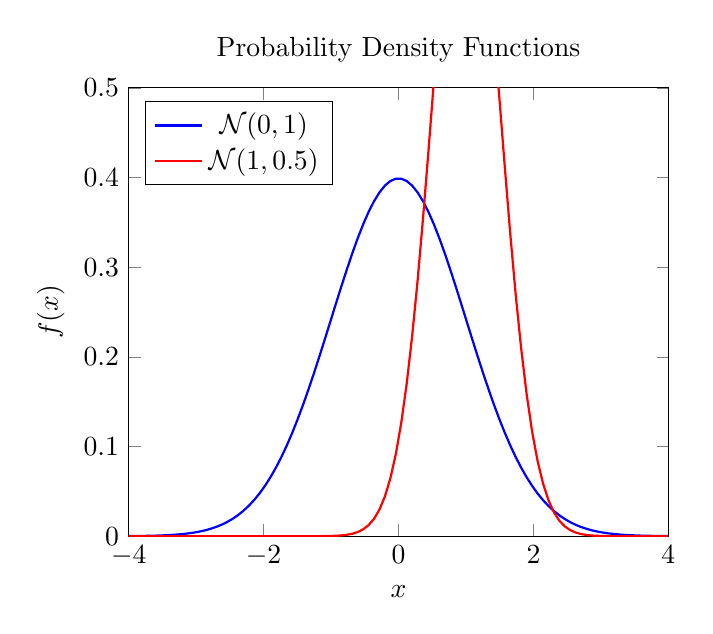
\begin{tikzpicture}
\begin{axis}[
    xlabel={$x$},
    ylabel={$f(x)$},
    xmin=-4, xmax=4,
    ymin=0, ymax=0.5,
    domain=-4:4,
    samples=100,
    legend pos=north west,
    title={Probability Density Functions}
]
\addplot[blue, thick] {1/sqrt(2*pi)*exp(-x^2/2)};
\addlegendentry{$\mathcal{N}(0, 1)$};
\addplot[red, thick] {1/sqrt(2*pi*0.5^2)*exp(-(x-1)^2/(2*0.5^2))};
\addlegendentry{$\mathcal{N}(1, 0.5)$};
\end{axis}
\end{tikzpicture}
\caption{Normal distributions with different parameters}
\end{figure}

\section{Properties and Relationships}
\subsection{Moment Generating Functions}
The moment generating function (MGF) of a random variable $X$ is defined as:

\begin{align}
M_X(t) = E[e^{tX}] = \int_{-\infty}^{\infty} e^{tx} f_X(x) dx
\end{align}

MGFs uniquely determine probability distributions and are useful for finding moments.

\subsection{Central Limit Theorem}
The central limit theorem states that the sum (or average) of a large number of independent, identically distributed random variables tends toward a normal distribution, regardless of the original distribution.

\subsection{Law of Large Numbers}
The law of large numbers states that as the number of identically distributed, randomly generated variables increases, their sample mean approaches their theoretical mean.

\section{Applications}
\subsection{Quality Control}
Binomial and normal distributions are used in statistical process control to monitor manufacturing processes.

\subsection{Reliability Engineering}
Exponential and Weibull distributions model failure rates and component lifetimes.

\subsection{Finance}
Log-normal distributions model stock prices, while normal distributions are used in option pricing models.

\subsection{Queuing Theory}
Poisson and exponential distributions model arrival rates and service times in queuing systems.

\section{Exercises}
\begin{enumerate}
    \item A fair coin is tossed 10 times. What is the probability of getting exactly 6 heads?
    \item The number of customers arriving at a bank follows a Poisson distribution with an average of 5 customers per hour. What is the probability that exactly 3 customers arrive in a one-hour period?
    \item If $X$ follows a normal distribution with $\mu = 70$ and $\sigma = 5$, find $P(65 < X < 75)$.
    \item A machine produces parts with lifetimes that follow an exponential distribution with a mean of 500 hours. What is the probability that a part will last more than 600 hours?
    \item Prove that the sum of two independent normal random variables is also normally distributed.
\end{enumerate}

\section{Further Reading}
\begin{itemize}
    \item Feller, W. (1968). An Introduction to Probability Theory and Its Applications.
    \item Casella, G., \& Berger, R. L. (2002). Statistical Inference.
    \item Ross, S. M. (2014). Introduction to Probability Models.
\end{itemize}

\end{document} 